\chapter{Experimental Results}
\label{experimental_results}
The real value in using sparsity for waveform inversion manifests through its application. Backed by an efficient implementation of the radar model operators and the quick convergence of tuned sparse recovery algorithms, we are primed to demonstrate the waveform inversion method on real radar data. Though the eventual goal in applying this technique is to enable highly-flexible and artifact-free measurements, the goals of this experiment are to \begin{inparaenum}[(1)]
 \item show that waveform inversion produces results that are consistent with our expectations,
 \item directly compare the effectiveness of different waveforms, and
 \item collect high-quality meteor data.
\end{inparaenum}

We expected that inversion would eliminate delay-frequency sidelobes and strictly improve upon matched filtering, and the experiment is successful in demonstrating that. We know that the pulse waveform directly affects measurement incoherence in terms of compressed sensing, and the experiment shows that successful inversion is dependent on the compactness of the peak of the waveform's ambiguity function. Regarding meteors, the hope was that eliminating sidelobes and increasing resolution through waveform inversion would allow us to address the open questions concerning flares and micrometeoroid fragmentation \autocite{MBMC10}. Further experimentation will be required to answer those questions, but the experiment proves that the technique is still useful for eliminating interference between meteor head echoes and stationary targets like non-specular trails and the equatorial electrojet. Without sidelobe interference, each of those phenomena can be detected more reliably and studied independently.

From February 28 through March 2, 2011, we collected approximately 48 hours of nearly-continuous data observing the equatorial ionosphere using the Jicamarca 50 MHz radar. That amounted to over two terabytes of receiver samples. Even with fast code and good algorithms, it is not reasonable at this time to apply the waveform inversion technique to anything more than tiny segments of that data. We have chosen to focus on a handful of examples collected from the Jicamarca data set in order to analyze them in detail and infer the method's effectiveness in general. With the knowledge gained from this experience, we are able make recommendations to aid future applications of the waveform inversion technique.

\section{Jicamarca}
\label{jicamarca_overview}
The Jicamarca 50 MHz radar is a phased array composed of 18,432 crossed half-wave dipoles in a 96 by 96 square grid (Figures \ref{fig:jicamarca} and \ref{fig:jicamarca_and_me}), covering an area of almost 85,000 square meters.
\begin{figure}[tbp]
 \centering
 %\includegraphics[width=0.75\textwidth,trim=0px 20px 0px 100px,clip]{fairuse/jicamarca}
 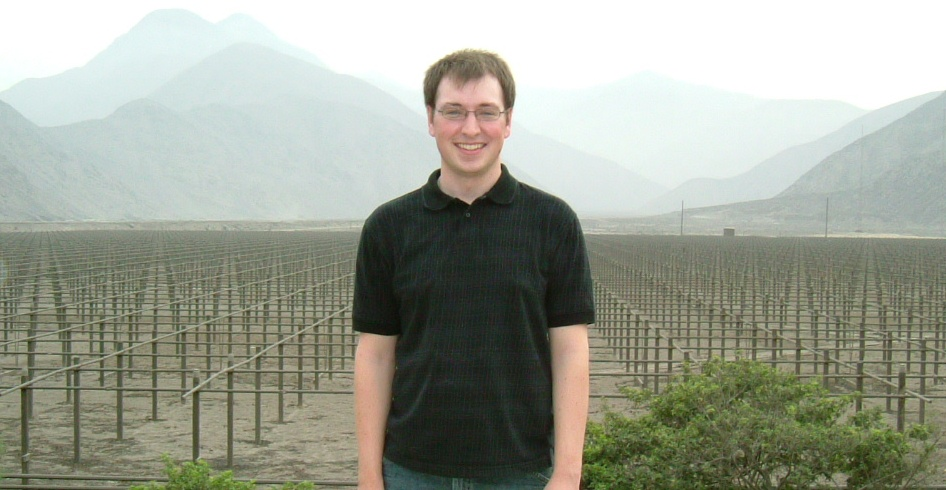
\includegraphics[width=0.75\textwidth]{jicamarca_and_me}
 \caption[The Jicamarca 50 MHz radar]{\emph{The Jicamarca 50 MHz radar.} The author is pictured, pre-experiment, in front of the Jicamarca Radio Observatory's main radar, a large phased array operating at 50 MHz and consisting of 18,432 crossed half-wave dipoles. Located outside of Lima, Peru, the radar's primary use is to study the equatorial ionosphere from its vantage point near the magnetic equator.}
 \label{fig:jicamarca_and_me}
\end{figure}%
It is located inland from Lima, Peru, at a geographic latitude and longitude of 11.95$^\text{o}$ south, 76.87$^\text{o}$ west, placing it near the magnetic equator \autocite{Och63}. Accordingly, the main use of Jicamarca is the study of the equatorial ionosphere, and monitoring its background plasma through incoherent scatter is one primary objective. Since the radar is able to point perpendicular to the Earth's magnetic field (or nearly so), it enjoys a number of rare capabilities. Ultra-precise measurement of ionospheric electric fields is one benefit of that configuration, as is the ability to view field aligned irregularities, which are frequently fueled by meteor ionization and radar-visible as non-specular meteor trails \autocite{WH69, CK94}. The study of these and other unique transient events, including spread-F and the equatorial electrojet, is another focus of Jicamarca's scientific program. Thanks to the radar's low VHF frequency relative to other high-power large-aperture (HPLA) radars, more meteor head echoes are detectable with the Jicamarca array than with almost all of those other HPLAs given the inverse scaling of frequency with received signal strength, which scales approximately as $1/f^2$. Head echoes, trails, and electrojet are near-constant features of the daytime ionosphere at Jicamarca. This crowded and challenging environment is a great proving ground for new measurement techniques, and it provides a surfeit of opportunities for testing our waveform inversion method.

\subsection{Specifications}
The observatory is currently equipped with three transmitters that each have a peak power output of about 1.5 MW, for a total possible transmitter power of 4.5 MW. The transmitter system supports a variety of pulsed waveforms, including binary-phase codes and the LFM chirp. These pulses can be transmitted with a maximum duty cycle of 6\%, a maximum bandwidth of about 1 MHz (shortest pulse of 1 microsecond), and a maximum length of 2 milliseconds. Four phase-coherent receivers can be used to sample the acquired signal with a maximum bandwidth of 1 MHz. Each receiver downmixes the signal to baseband frequency and outputs complex samples representing in-phase and quadrature components \autocite{JICAMARCA_SPEC}.

\subsection{Array Segmentation}
The four receiver channels can measure signals from distinct subsets of the whole array. One typical configuration involves sampling the four quadrants of the array independently. Comparison of signal phase between these quadrants through interferometry allows one to determine the signal's direction of arrival. The channels can also be used to sample independent polarizations or more complex interferometry setups with multiple measurement baselines. The dipoles are actually organized into 64 separate, square modules; the modules can be sampled in any combination, but they can also be phased independently to form different beam patterns. Tuned appropriately, the full array has a one-way half power beamwidth (full-width at half maximum) of 1.1$^\text{o}$ and can be electronically steered within about 7$^\text{o}$ of zenith. Currently, individual module phasing must be carried out manually by adjusting cable lengths, but a computer-controlled phasing system is being developed to enable pulse-to-pulse beam pointing \autocite{JICAMARCA_SPEC}.

\section{Setup}
The suitability of different radar waveforms for sparse recovery is an open question. We expect from theoretical results that random or pseudorandom waveforms will produce suitably incoherent measurements, but most of the standard waveforms also merit investigation. Because they are designed to minimize the effects of ambiguity, codes with ideal sidelobe properties are likely to also be useful for inversion. Our experiment using the Jicamarca radar was designed to test the effectiveness of a number of these common waveforms by comparing them side-by-side while scattering from the same targets. Switching the code on a pulse-to-pulse basis allows us to judge waveforms against each other under the same circumstances. As long as we eventually repeat the same waveform after a short time relative to the persistence of the target, we can build up equivalent views of a radar scene using a number of different waveforms.

\subsection{Waveforms}
For this experiment, we selected five different waveforms and stepped through them sequentially before repeating the sequence. The five waveforms are depicted using a meteor head and trail in Figure \ref{fig:waveform_sequence}; the waveforms are, in order, a Barker-13 code (B$_\text{13}$), a minimum peak sidelobe code (MSL$_\text{51}$), an uncoded pulse, a linear frequency modulation (LFM) chirp, and a pseudorandom code (PSRND$_\text{51}$).
\begin{figure}[tpb]
 \centering
 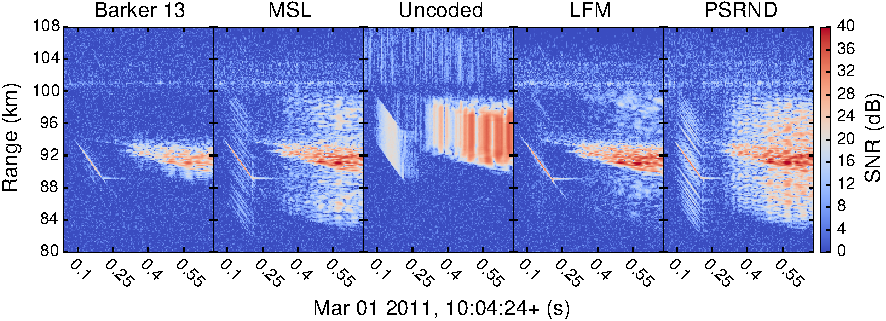
\includegraphics{head_and_flare_mf_rti_block}
 \caption[Sequence of waveforms used in the Jicamarca experiment]{\emph{Sequence of waveforms used in the Jicamarca experiment.} The images show example meteor data collected with the Jicamarca radar using five different pulse waveforms. The radar transmits just one of the five waveforms with each pulse, stepping through the sequence of five in the order shown before repeating.}
 \label{fig:waveform_sequence}
\end{figure}%
The first four were chosen because they are widely used for collecting meteor head echo and trail data \autocite{WPW96, ELWF01, MBMH08, COHD02}. The pseudorandom code was chosen because it was expected to have good waveform inversion performance based on compressed sensing theory \autocite{BSN08, PR10}. The three binary phase codes are described by the following sequences:
\begin{align}
 s_{\text{B}_\text{13}} &= 1111100110101\nonumber\\
 s_{\text{MSL}_\text{51}} &= 000111000111111100010001100100010010101001001001011\nonumber\\
 s_{\text{PSRND}_\text{51}} &= 011111000010000001001100001011000001001011010011100\nonumber.
\end{align}

\subsection{Pulse Parameters}
With the exception of the uncoded pulse, a bandwidth of 1 MHz (the maximum at Jicamarca) was fixed as the primary design point. A high bandwidth equates to better pulse compression and smaller regions of ambiguity. For the phase-coded pulses, that requirement specifies a baud length of 1 $\mu$s. For the LFM chirp, it specifies a total frequency sweep of 1 MHz, centered around the radar frequency. The Barker-13 code is the longest binary code with a maximum sidelobe level of 1 when the peak is normalized to the code length, but it is still short, with a total pulse length of 13 $\mu$s, compared to the other pulses. We wanted a longer minimum peak sidelobe code in order to test the effects of pulse length, so the code of length 51 was chosen since it is the longest that has a peak sidelobe level of 3 or less. Hence, the MSL$_\text{51}$ pulse has a length of 51 $\mu$s. The lengths of the LFM and pseudorandom pulses were chosen to match the minimum sidelobe pulse. The pseudorandom code was indeed produced by a random number generator; we drew a few binary codes of length 51 until we found one with a somewhat-uniform autocorrelation. Finally, the uncoded pulse bears almost no relation to the others. It was included as a baseline so that any unusual results from the coded pulses could be compared to the simplest data possible. A length of 40 $\mu$s was arbitrarily chosen to be long enough for reasonable sensitivity but short enough for reasonable ambiguity, and it is close to the value used by \textcite{MDW+03} at Arecibo.

\subsection{Pulse Timing}
Meteors are typically observed at altitudes ranging from 80 to 120 kilometers, although they are sometimes observed as low as 70 kilometers and as high as 140 kilometers. With that as our primary range window of interest, we chose an inter-pulse period of 1.02 ms, with the corresponding maximum unambiguous range of 153 km, to minimize the time required to repeat the waveform sequence. It is advantageous to repeat each waveform as quickly as possible to ensure that even transient events would be sampled sufficiently by each type of pulse. This is also the reason that the waveform sequence was limited to five pulses. With that inter-pulse period, the longest pulses in our pulse sequence nearly achieve the maximum duty cycle of Jicamarca's transmitter.

\subsection{Sampling}
High resolution is an obvious goal for meteor measurements so that accurate range and range rate estimates are possible. Waveform inversion is also dependent on having enough measurements relative to the sparsity level to ensure success. The highest sampling rate is desirable, and at Jicamarca that means a sampling period of 1 $\mu$s. With the selected waveforms consuming 1 MHz of bandwidth and switching phases at a period of 1 $\mu$s, no other choice would have made sense.

\section{Procedure}
\label{waveform_inversion_procedure}
The waveform inversion procedure specified in Section \ref{waveform_inversion_solution} was applied to second-long windows of the Jicamarca data. To ensure proper normalization for inversion, the radar model was defined with the code sequence $s$ normalized to a power of 1. To ensure that the number of frequency steps exceeded the length of the longest code sequences, the number of frequency steps $N$ was set at 128. Specifying a power of 2 ensures maximally-efficient Fourier transforms, and the higher value ensures just enough frequency resolution to differentiate moving head echoes from stationary targets. Except where noted, the model was defined with no undersampling, $R=1$. In all cases, we used the accelerated proximal gradient method with adaptive restart and adaptive step size to iteratively solve for the sparse reflectivity from the measurements. Each pulse was analyzed individually, with no shared information other than the uniformly-specified regularization parameter $\lambda$, which was set based on the estimated noise level. Using a recent laptop computer to perform the computations, the solution for each one-second segment of data took anywhere from 15 minutes to 1 hour to calculate. For a single pulse, the solution converged in approximately 1 second, with denser solutions taking correspondingly longer.

\section{Pseudorandom Pulse Results}
\label{pseudorandom_results}
Given the theoretical backing, it was expected that the pseudorandom waveform would be suitable for inversion. Fortunately, that is the case. Many of the waveform inversion features of the pseudorandom code are shared by the other waveforms. Therefore, we can summarize many of the basic features of the technique by first limiting our attention to the pseudorandom pulses.

\subsection{Pulse Slices}
Figures \ref{fig:head_timeslice} and \ref{fig:trail_timeslice} compare waveform inversion and matched filter bank results over a series of individual pseudorandom pulses.
\begin{figure}[tpb]
 \centering
 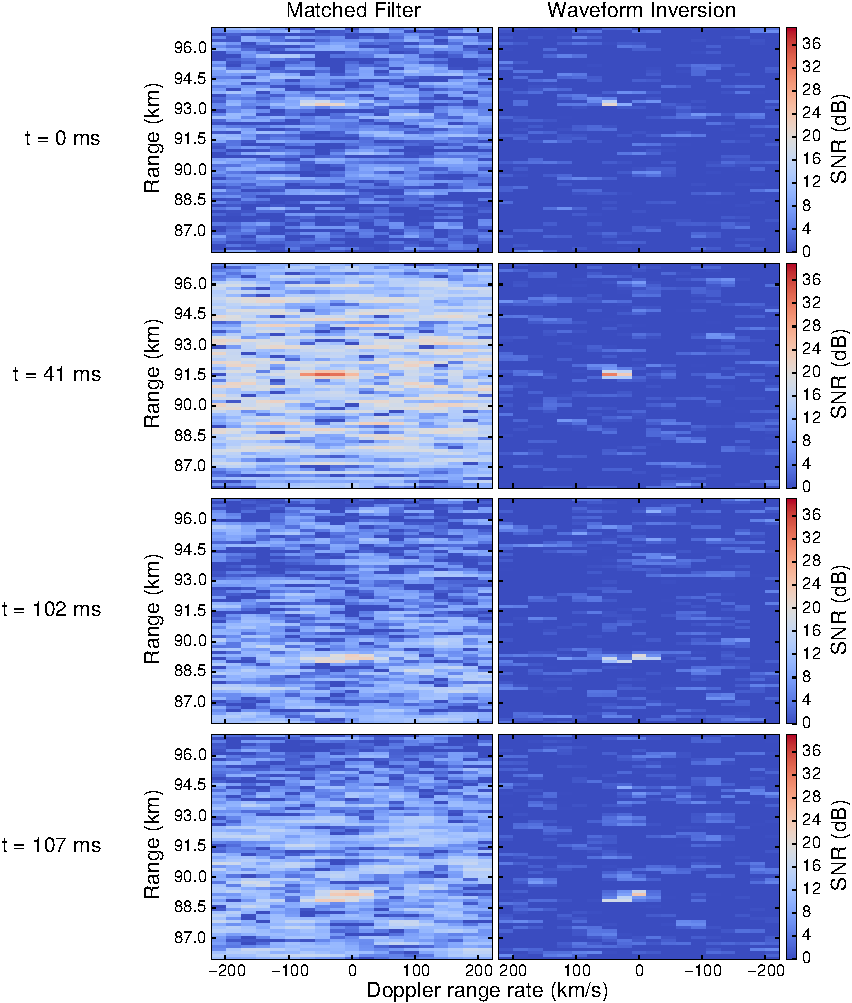
\includegraphics{head_and_flare_mf_vs_recovered_p4_ts20}
 \caption[Pulse slices comparing matched filter and waveform inversion]{\emph{Pulse slices comparing matched filter and waveform inversion.} The images in each row depict meteor head echo scattering as a function of range (delay) and Doppler range rate (frequency) for a single pseudorandom pulse. Corresponding pulse times, relative to the first pulse, are shown at left. The differentiated signal in the waveform inversion result (right column), somewhat obscured in the matched filter result (left column), shows the head echo descending in range and flaring.}
 \label{fig:head_timeslice}
\end{figure}%
\begin{figure}[tpb]
 \centering
 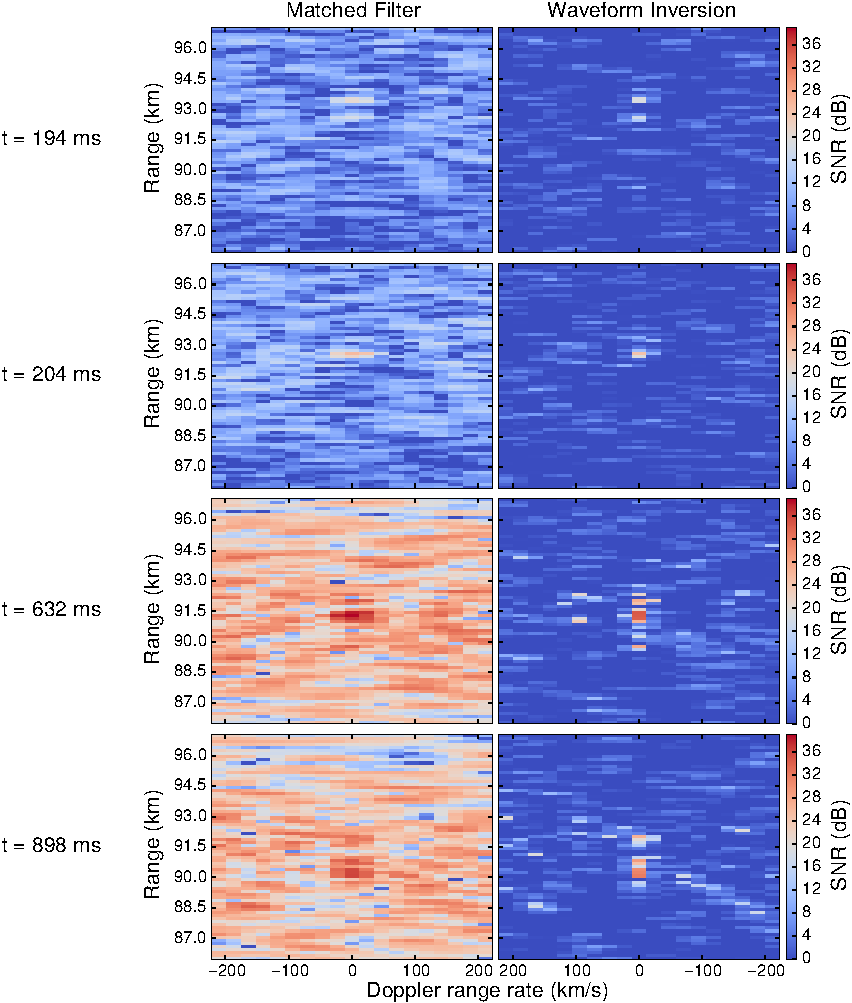
\includegraphics{head_and_flare_mf_vs_recovered_p4_ts52}
 \caption[Pulse slice comparison for a meteor trail]{\emph{Pulse slice comparison for a meteor trail.} The images in each row depict non-specular trail scattering as a function of range (delay) and Doppler range rate (frequency) for a single pseudorandom pulse. Corresponding pulse times, relative to the time of the first pulse shown in Figure \ref{fig:head_timeslice}, are shown at left. Waveform inversion (right column) removes the sidelobes obscuring the matched filter result (left column) to make the fluctuating scattering at zero-range rate clearly visible.}
 \label{fig:trail_timeslice}
\end{figure}%
Each slice represents data from a single pulse and shows part of the delay-frequency decomposition of the radar signal, giving SNR as a function of range and Doppler range rate. Figure \ref{fig:head_timeslice} shows the time evolution of a meteor head echo that ends in a flare. The head echo is first visible as a single point with negative range rate coming toward the radar, and over time it descends in range until flaring and exiting the radar beam. Figure \ref{fig:trail_timeslice} depicts the initial appearance and later fluctuation in the non-specular trail that follows the head echo. The scattering has a Doppler range rate of zero and fades in and out over the ranges containing the meteor plasma, according to the scattering characteristics of the evolving field-aligned irregularities.

The range rate axis has particularly poor resolution for these and all of the other results. The meteor head echo, traveling at approximately 40 km/s toward the radar, is only two range rate/frequency steps away from zero out of the 128 total grid points. This is a result of Jicamarca's relatively low baseband frequency of 50 MHz. At that frequency, even fast moving targets can barely generate a significant frequency shift relative to the available pulse lengths. Better frequency/range rate resolution is only possible by increasing the length of time covered by the frequency analysis, and that means analyzing the same target over multiple pulses. As such, the frequency resolution cannot be improved without the development of a multi-pulse waveform inversion technique.

Though it makes no practical difference for a single point target like the meteor head echo, the first thing to notice from the results is just how significant the delay-frequency sidelobes are in the matched filter solution. Waveform inversion effectively eliminates those sidelobes, leaving only the head echo points and noise, the latter of which has been added back to the sparse solution from the residual. It is also important to note the second row of head echo images, in which the solitary target appears to occupy multiple points spanning two range rate bins. This is as expected for a point target, due to the blurring experienced as a result of discretization (see Section \ref{point_target_reflectivity}). The true range rate lies between those two grid points, and the discrete model copes by spreading the signal over both. The flaring seen in the last two rows of head echo images is notable because sidelobe removal allows us a clearer view of the signal, which can be seen spreading to zero range rate while the head echo continues to descend. Given the poor frequency resolution, it is impossible to draw any conclusions from this result, but it is a good illustration of a potential future application.

The non-specular meteor trail is most notable for how the results go from completely cluttered in the matched filter case to relatively clean in the waveform inversion case, all thanks to the elimination of sidelobes. The most significant scattering is still noticeable with the matched filter, but it is also impossible to tell if the rest represents actual scattering or just delay-frequency sidelobes. Waveform inversion answers that question by clearly separating true scattering from sidelobe. Nevertheless, the waveform inversion solution is not perfect. It includes some significant signal at impossibly high frequencies/range rates, which we are inclined to identify as reconstruction artifacts. The best guess is that the artifacts represent the result of the transmitted signal not exactly matching the ideal, infinite-bandwidth code used in the model. As a result, the sparse solution is forced to include whatever coefficients add together to make up the difference between the actual and expected pulse shape. Imperfect matching is sufficient for good pulse compression, but the difference is much harder to account for in the sidelobes.

\subsection{Integrated RTI Plots}
The same meteor head echo, flare, and trail is shown in Figure \ref{fig:mf_vs_recovered_rti} as a range-time-intensity (RTI) plot.
\begin{figure}[tpb]
 \vspace{-1.5\baselineskip}
 \begin{subfigure}{\textwidth}
  \centering
  \textsf{\footnotesize Mar 01 2011, 10:04:xx (s)}
  
  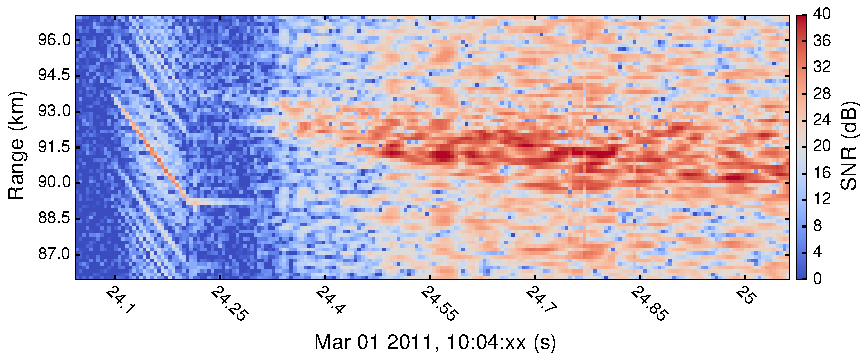
\includegraphics[trim=0px 20px 0px 3px,clip]{head_and_flare_mf_rti_4}
  \caption{Matched filter}
  \label{fig:example_mf_rti}
 \end{subfigure}
 
 \vspace{0.5\baselineskip}
 \begin{subfigure}{\textwidth}
  \centering
  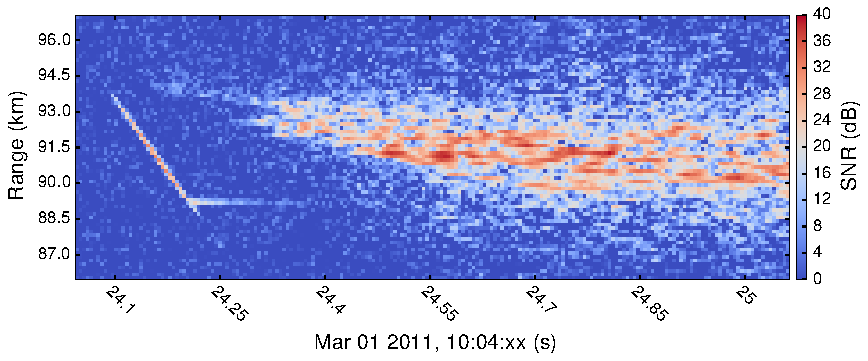
\includegraphics[trim=0px 20px 0px 3px,clip]{head_and_flare_recovered_rti_noise_4}
  \caption{Waveform inversion}
  \label{fig:example_recovered_rti}
 \end{subfigure}
 \caption[RTI comparison of matched filter and waveform inversion]{\emph{RTI comparison of matched filter and waveform inversion.} These images show the same pseudorandom-coded meteor head, flare, and trail from Figures \ref{fig:head_timeslice} and \ref{fig:trail_timeslice}. The matched filter result is for the peak-frequency-response of each pulse, while the waveform inversion result is the integrated power over all frequency coefficients. The elimination of delay-frequency sidelobes with waveform inversion reveals previously-obscured trail scattering and makes the true signal easier to identify.}
 \label{fig:mf_vs_recovered_rti}
\end{figure}%
The matched filter result in part (\subref{fig:example_mf_rti}) is for the peak-frequency-response filter for each individual pulse, selected from the entire frequency bank of 128 filters. The waveform inversion result in part (\subref{fig:example_recovered_rti}) is for the total signal summed across all frequency coefficients, which is sensible only because no delay-frequency sidelobes are present. The sparse solution's residual was matched filtered and added to the sparse coefficients to form the waveform inversion result as described in Section \ref{waveform_inversion_solution}.

As with the time slices of this data, waveform inversion is notable for removing the range sidelobes that clutter the matched filter result while retaining the high SNR of the true signal. There can be no doubt here that the waveform inversion method is beneficial. The pseudorandom code's autocorrelation function is clearly visible in the matched filter image, surrounding the descending head echo streak. With waveform inversion, those range sidelobes are completely eliminated to reveal previously-obscured trail scattering. Much of the clutter is also removed for the non-specular trail, although some artifacts remain. As previously discussed, these artifacts are likely the result of mismatch between the actual pulse waveform and its idealized representation in the radar model. Even with these artifacts, the result is much improved.

\subsection{Frequency Slices}
One way to minimize the effect of recovery mismatch artifacts is to analyze the individual frequency slices of the waveform inversion result. Frequency decomposition also makes it easy to separate and identify different types of signals. It is generally not possible to perform this type of analysis with a matched filter, since sidelobes of one target often obscure the features of another target even when separated in frequency. To demonstrate, Figure \ref{fig:recovered_dopplerslices} shows the first three positive frequency shifts, starting at zero, of the previous waveform inversion result.
\begin{figure}[tpb]
 \vspace{-1.5\baselineskip}
 \begin{subfigure}{\textwidth}
  \centering
  \textsf{\footnotesize Mar 01 2011, 10:04:xx (s)}
  
  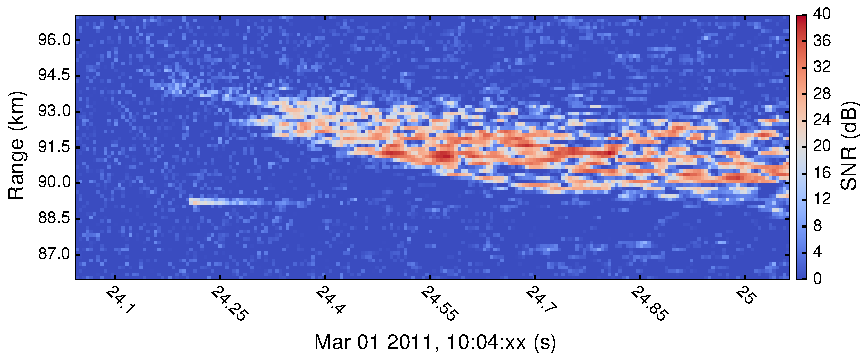
\includegraphics[trim=0px 20px 0px 3px,clip]{head_and_flare_recovered_doppler_rti_f0_p4}
  \caption{Zero frequency shift}
  \label{fig:recovered_dopplerslices_f0}
 \end{subfigure}
 
 \vspace{0.5\baselineskip}
 \begin{subfigure}{\textwidth}
  \centering
  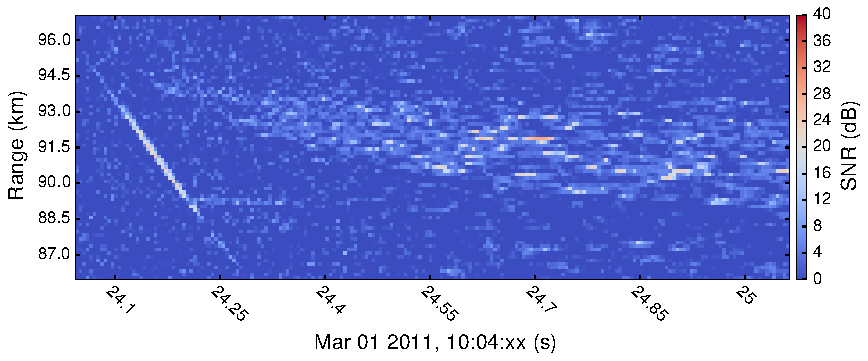
\includegraphics[trim=0px 20px 0px 3px,clip]{head_and_flare_recovered_doppler_rti_f1_p4}
  \caption{1st frequency step, 7.8 kHz shift ($-$23.4 km/s)}
  \label{fig:recovered_dopplerslices_f1}
 \end{subfigure}
 
 \vspace{0.5\baselineskip}
 \begin{subfigure}{\textwidth}
  \centering
  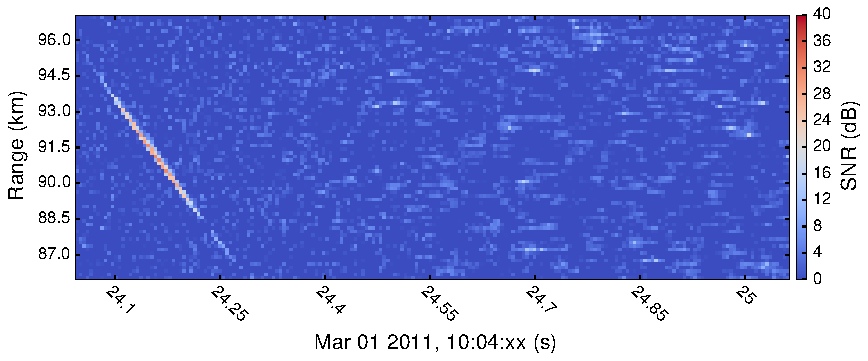
\includegraphics[trim=0px 20px 0px 3px,clip]{head_and_flare_recovered_doppler_rti_f2_p4}
  \caption{2nd frequency step, 15.6 kHz shift ($-$46.9 km/s)}
  \label{fig:recovered_dopplerslices_f2}
 \end{subfigure}
 \caption[Frequency slices of waveform inversion]{\emph{Frequency slices of waveform inversion.} These images show the same meteor head, flare, and trail from Figure \ref{fig:mf_vs_recovered_rti} decomposed over the first three frequency steps of the waveform inversion result. The stationary flare and trail appear in the zero-frequency slice, while the moving head echo appears at positive frequency shifts.}
 \label{fig:recovered_dopplerslices}
\end{figure}%

As nearly stationary targets, meteor trails exhibit only a small Doppler shift that is on the order of 100 m/s and is associated with the background neutral winds. Because this potential shift is very small compared to the waveform inversion frequency resolution, the flare and non-specular trail are clearly visible in the zero-frequency result. In contrast to the frequency-integrated RTI plot, the trail as shown at zero frequency is free from clear mismatch artifacts. The artifacts are spread randomly throughout the entire frequency space, so it is reasonable that they would not be very noticeable in any one frequency slice. The meteor head echo is visible in the image showing the first positive frequency shift, 7.8 kHz or $-$23.4 km/s in Doppler range rate. Although the true meteoroid velocity is higher, frequency spreading from discretization causes the signal to appear in this neighboring slice. A faint background of the trail is also visible in this image, along with a few points of higher SNR. The ghost trail is due to the frequency ambiguity of the code, and it appears as a result of applying the matched filter to the sparse solution's residual. This step is necessary to de-bias the sparse result and restore the signal that was shrunk toward zero. The second frequency step, 15.6 kHz or $-$46.9 km/s, is closest to the Doppler range rate of the head echo, and so its signal is strongest in the third plot. For the first time, we can also see that the head echo continues after disappearing for a few pulses; this is most likely due to the meteor exiting the main radar beam and reappearing in an antenna sidelobe. It is impossible to identify this feature in the matched filter or even the frequency-integrated result, but frequency decomposition allows us to find it. The absence of trail signal at the second frequency step is also reassuring, lending support to the theory that the signal seen in the first step is due to discretization spreading.

\subsection{Sparse Solution and Residual}
Next we investigate the separate sparse and measurement residual terms that form the waveform inversion result. The composition of the zero-frequency slice of the previous meteor example is shown in Figure \ref{fig:recovered_solution_composition}.
\begin{figure}[tpb]
 \vspace{-1.5\baselineskip}
 \begin{subfigure}{\textwidth}
  \centering
  \textsf{\footnotesize Mar 01 2011, 10:04:xx (s)}
  
  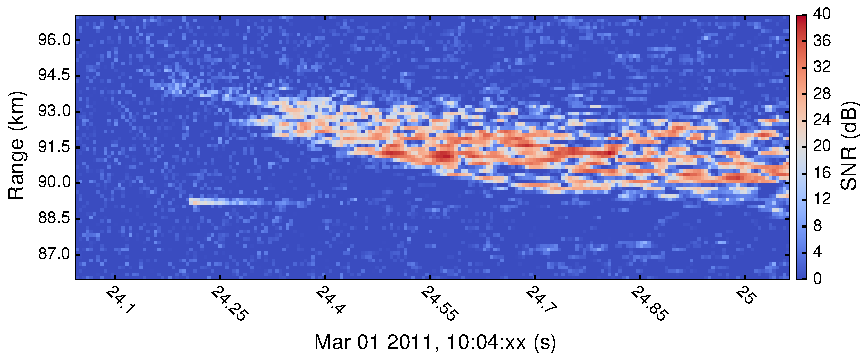
\includegraphics[trim=0px 20px 0px 3px,clip]{head_and_flare_recovered_doppler_rti_f0_p4}
  \caption{Waveform inversion combining sparse solution and residual}
  \label{fig:recovered_total}
 \end{subfigure}
 
 \vspace{0.5\baselineskip}
 \begin{subfigure}{\textwidth}
  \centering
  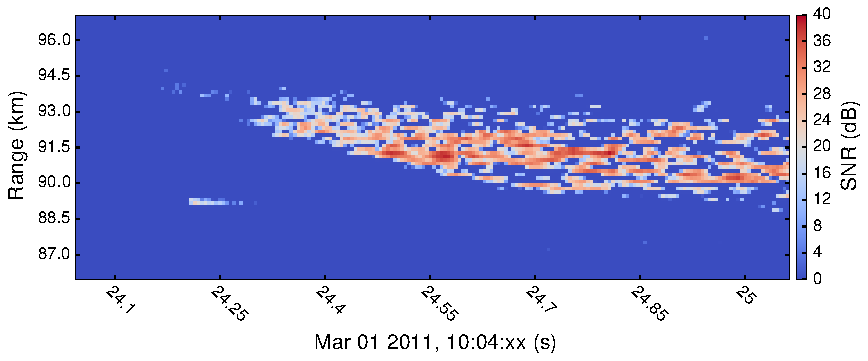
\includegraphics[trim=0px 20px 0px 3px,clip]{head_and_flare_recovered_sparse_doppler_rti_f0_p4}
  \caption{Sparse solution}
  \label{fig:recovered_sparse}
 \end{subfigure}
 
 \vspace{0.5\baselineskip}
 \begin{subfigure}{\textwidth}
  \centering
  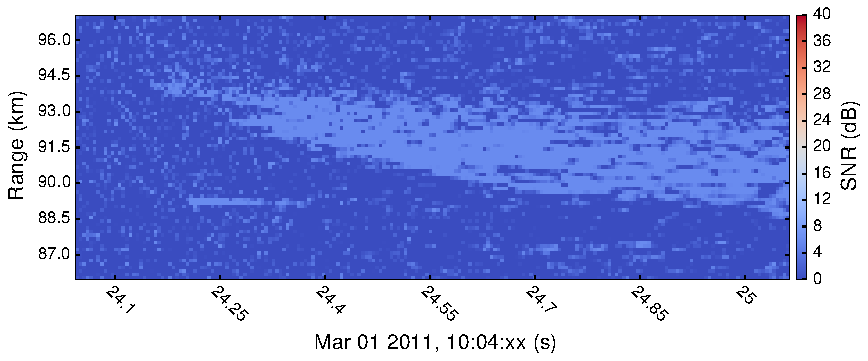
\includegraphics[trim=0px 20px 0px 3px,clip]{head_and_flare_recovered_noise_doppler_rti_f0_p4}
  \caption{Matched filtered measurement residual}
  \label{fig:recovered_noise}
 \end{subfigure}
 \caption[Decomposition of waveform inversion as sparse and residual solutions]{\emph{Decomposition of waveform inversion as sparse and residual solutions.} The sparse solution is found by minimal $l_1$ fitting to the radar model, while the residual term is formed by matched filtering the remaining measurement error. Both contain important features that are added together to compose the waveform inversion solution.}
 \label{fig:recovered_solution_composition}
\end{figure}%
Figure \ref{fig:recovered_total} repeats the complete waveform inversion image, while Figures \ref{fig:recovered_sparse} and \ref{fig:recovered_noise} show the sparse and residual components.

As expected, the sparse solution contains all of the significant coefficients that represent the flare and trail scattering. It is truly sparse, with most of the shown zero-frequency coefficients and the vast majority of the unshown nonzero-frequency coefficients equal to zero. The sparse solution is excellent for identifying targets and examining the high-SNR components, but it does not provide all of the needed information. Since the sparse solution by itself is biased toward zero, the residual contains not only noise but also remaining elements of the signal that fall below the detection threshold. The additional signal that is necessary to de-bias the sparse solution is clearly visible for the flare and trail. This low-SNR element also includes crucial details like the initial formation of the trail and the continuation of the flare. Since it is matched filtered, the residual also contains sidelobes for that signal, but the sidelobes are necessarily so far below the noise level that they are inconsequential. When combined together into the waveform inversion result, all of the relevant features of the signal are visible for easy comparison and analysis. Nevertheless, it is still important to remember how those elements were formed.

\subsection{Detection Sensitivity}
In Figure \ref{fig:longtrail_recovery_rti_comparison}, we show RTI images for a different meteor in order to lend more support to our waveform inversion observations.
\begin{figure}[tpb]
 \vspace{-1.5\baselineskip}
 \begin{subfigure}{\textwidth}
  \centering
  \textsf{\footnotesize Mar 01 2011, 10:09:xx (s)}
  
  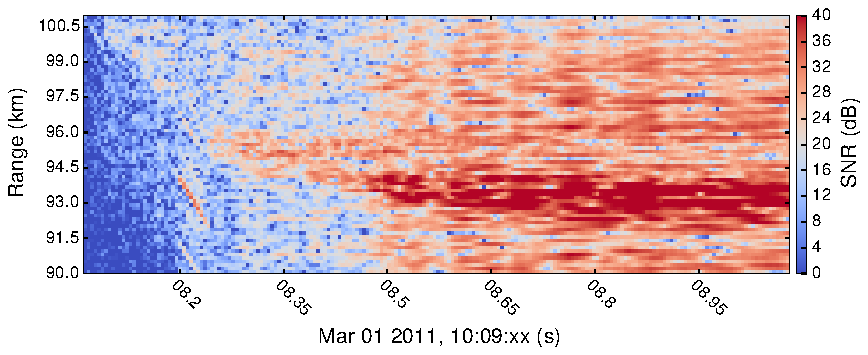
\includegraphics[trim=0px 20px 0px 3px,clip]{longtrail_mf_rti_4}
  \caption{Matched filter}
  \label{fig:longtrail_mf_rti}
 \end{subfigure}
 
 \vspace{0.5\baselineskip}
 \begin{subfigure}{\textwidth}
  \centering
  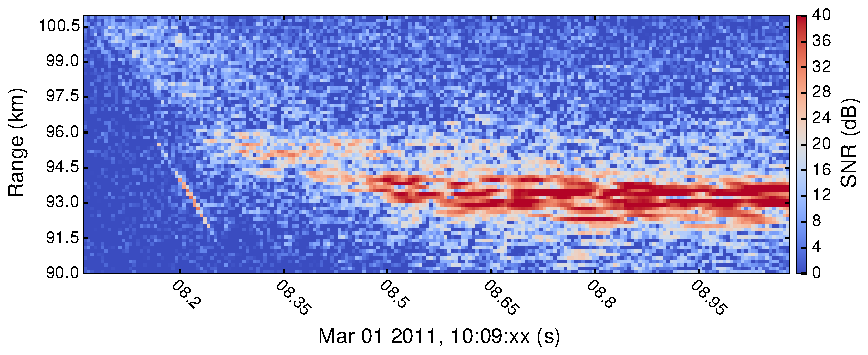
\includegraphics[trim=0px 20px 0px 3px,clip]{longtrail_recovered_rti_noise_4}
  \caption{Waveform inversion}
  \label{fig:longtrail_recovered_rti}
 \end{subfigure}
 
 \vspace{0.5\baselineskip}
 \begin{subfigure}{\textwidth}
  \centering
  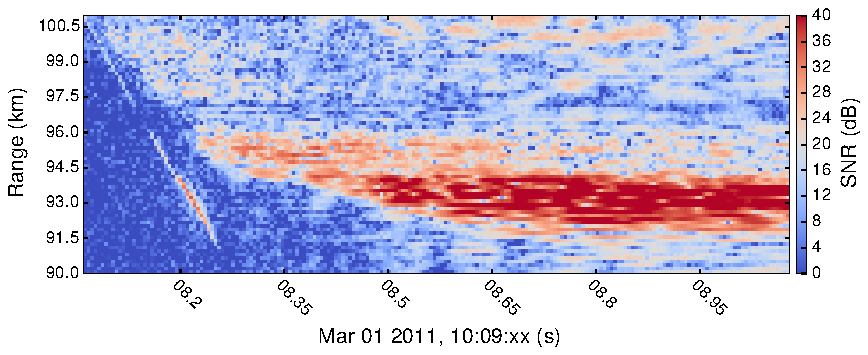
\includegraphics[trim=0px 20px 0px 3px,clip]{longtrail_mf_rti_3}
  \caption{Matched filter for LFM chirp}
  \label{fig:longtrail_mf_lfm_rti}
 \end{subfigure}
 \caption[Waveform inversion example for a different meteor]{\emph{Waveform inversion example for a different meteor.} The method is successful even with head echo and non-specular trail signals overlapping in the same pulse. This comparison includes the matched filter result for the neighboring LFM chirp pulses, which does a better job of differentiating the head echo.}
 \label{fig:longtrail_recovery_rti_comparison}
\end{figure}%
The matched filter result for the pseudorandom code is shown, followed by the corresponding waveform inversion result. A third image showing the matched filter result for the LFM chirp is also given in order to compare detection of the entire head echo. The overall conclusion taken from this data is the same as that from the previous example: waveform inversion is very successful at eliminating sidelobes and making obscured features visible, but it can also include artifacts from waveform mismatch. Comparison with the LFM chirp, which features the best matched filter results due to its unique delay-frequency ambiguity, reveals something new: signals with lower SNR are not always recoverable with a given waveform. The head echo is longer and better-defined with the LFM chirp. Waveform inversion makes more of the head echo evident than what is visible with the comparable matched filter, but we have clear evidence that it is possible to do better. The loss of signal on the head echo could just be due to actual- and ideal-code mismatch, but it is at least something to note for analyzing other results. Overall, waveform inversion with the pseudorandom code gives results that are clearly superior to the LFM chirp.

\section{Waveform Comparison Results}
In this section we compare the inversion performance of the various waveforms used in the Jicamarca experiment. Our results show that the success of the technique depends primarily upon the waveform's ambiguity function, but the quality of the recovery is more sensitive to pulse length and the fidelity of the transmitted waveform to its idealized representation.

\subsection{Minimum Peak Sidelobe Code}
The minimum peak sidelobe code enables waveform inversion with as much success as the pseudorandom code. Their identical length means that they should be able to recover signals with the same sensitivity, but it is reassuring to know that the minimum sidelobe code is suitably incoherent. The original meteor example returns in Figure \ref{fig:msl_comparison} with a comparison between the matched filter, frequency-integrated waveform inversion, and zero-frequency waveform inversion results.
\begin{figure}[tpb]
 \vspace{-1.5\baselineskip}
 \begin{subfigure}{\textwidth}
  \centering
  \textsf{\footnotesize Mar 01 2011, 10:04:xx (s)}
  
  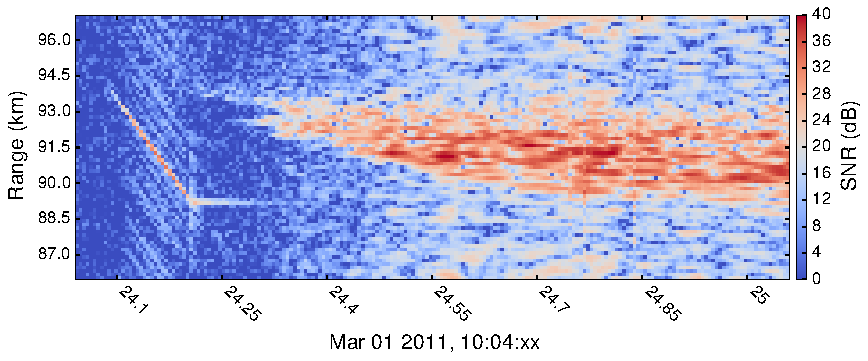
\includegraphics[trim=0px 20px 0px 3px,clip]{head_and_flare_mf_rti_1}
  \caption{Matched filter}
  \label{fig:msl_mf}
 \end{subfigure}
 
 \vspace{0.5\baselineskip}
 \begin{subfigure}{\textwidth}
  \centering
  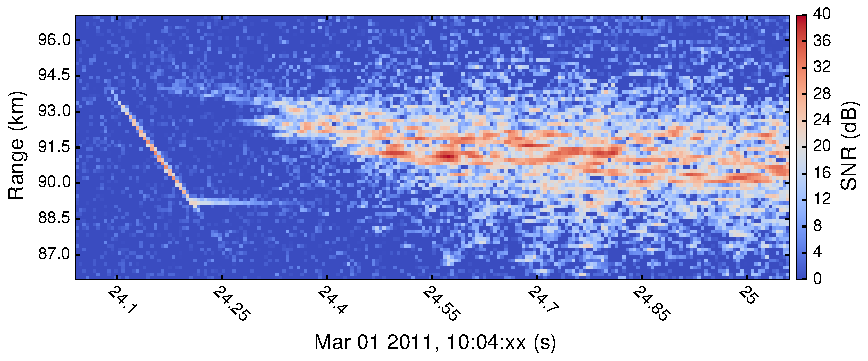
\includegraphics[trim=0px 20px 0px 3px,clip]{head_and_flare_recovered_rti_noise_1}
  \caption{Frequency-integrated waveform inversion}
  \label{fig:msl_recovered}
 \end{subfigure}
 
 \vspace{0.5\baselineskip}
 \begin{subfigure}{\textwidth}
  \centering
  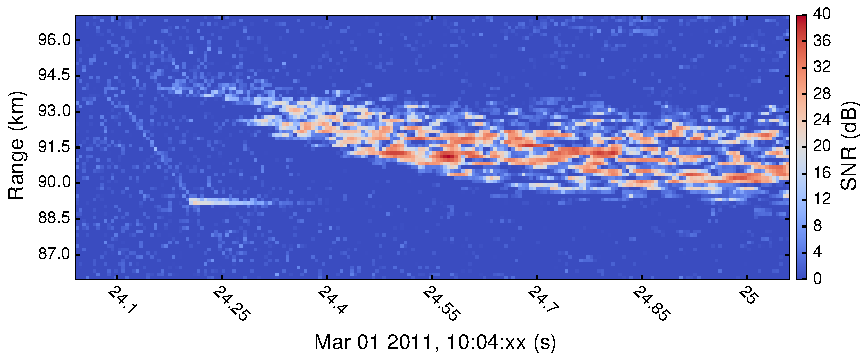
\includegraphics[trim=0px 20px 0px 3px,clip]{head_and_flare_recovered_doppler_rti_f0_p1}
  \caption{Zero-frequency slice of waveform inversion}
  \label{fig:msl_recovered_dopplerslice}
 \end{subfigure}
 \caption[Waveform inversion with the minimum peak sidelobe code]{\emph{Waveform inversion with the minimum peak sidelobe code.} With its good sidelobe properties, the minimum sidelobe code also demonstrates successful waveform inversion. Sidelobes are eliminated to provided a cleaner image, although the frequency-integrated result still suffers from mismatch artifacts.}
 \label{fig:msl_comparison}
\end{figure}%
Aside from a little leakage of the head echo into the zero-frequency result, the minimum sidelobe results exhibit the same features as the pseudorandom results. Given the better range sidelobe properties of the optimal minimum sidelobe code, one might hope that it might somehow be able to do better than pseudorandom code. While this may still be the case for scenes that push the sparsity limit, the difference between the codes is inconsequential in this case. This fact is not entirely surprising either, since the complete set of delay-frequency sidelobes for the minimum sidelobe code are not necessarily any more suitable for waveform inversion than those of the pseudorandom code.

\subsection{Barker-13 Code}
The Barker-13 code also has good sidelobe properties, so we would expect it to find success as well. Given its shorter length, however, it is less sensitive and more likely to have signals lost in the noise. Figure \ref{fig:b13_comparison} provides the now-familiar comparison images between matched filtering and waveform inversion.
\begin{figure}[tpb]
 \vspace{-1.5\baselineskip}
 \begin{subfigure}{\textwidth}
  \centering
  \textsf{\footnotesize Mar 01 2011, 10:04:xx (s)}
  
  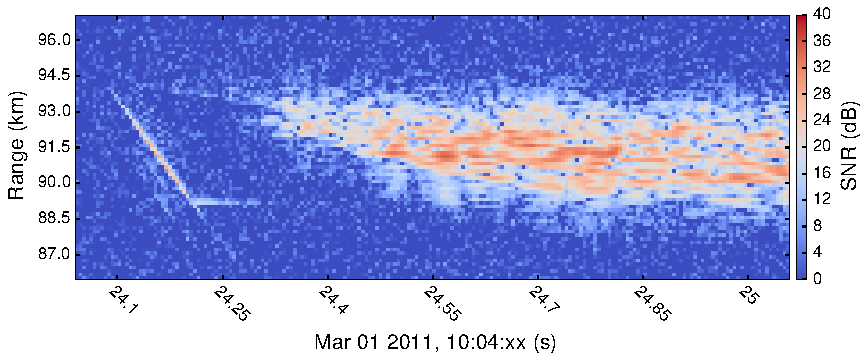
\includegraphics[trim=0px 20px 0px 3px,clip]{head_and_flare_mf_rti_0}
  \caption{Matched filter}
  \label{fig:b13_mf}
 \end{subfigure}
 
 \vspace{0.5\baselineskip}
 \begin{subfigure}{\textwidth}
  \centering
  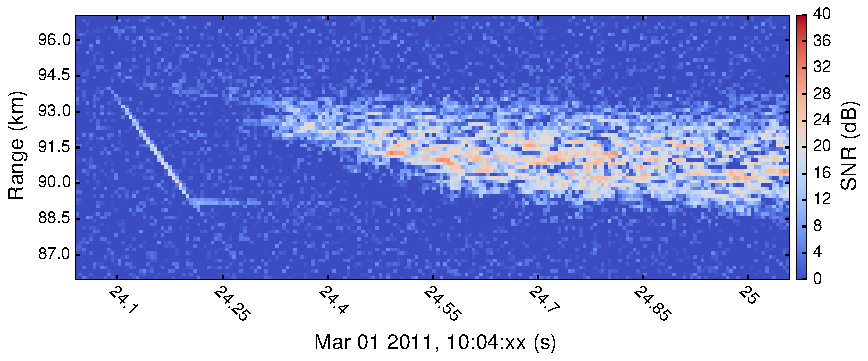
\includegraphics[trim=0px 20px 0px 3px,clip]{head_and_flare_recovered_rti_noise_0}
  \caption{Frequency-integrated waveform inversion}
  \label{fig:b13_recovered}
 \end{subfigure}
 
 \vspace{0.5\baselineskip}
 \begin{subfigure}{\textwidth}
  \centering
  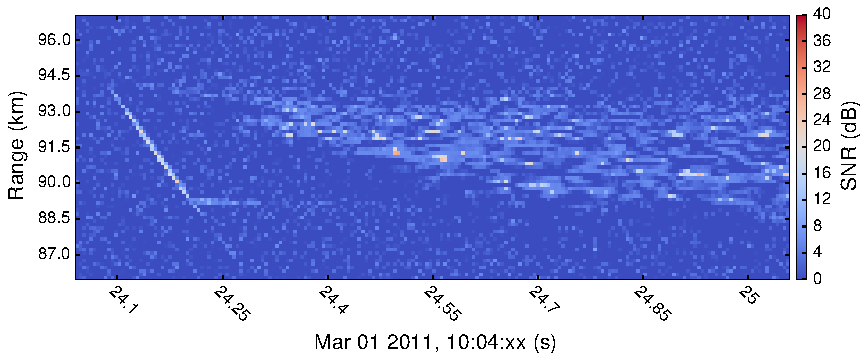
\includegraphics[trim=0px 20px 0px 3px,clip]{head_and_flare_recovered_doppler_rti_f2_p0}
  \caption{2nd frequency shift of waveform inversion, 15.6 kHz ($-$46.9 km/s)}
  \label{fig:b13_recovered_dopplerslice}
 \end{subfigure}
 \caption[Waveform inversion with the Barker-13 code]{\emph{Waveform inversion with the Barker-13 code.} The technique is moderately successful with the Barker-13 code. It effectively eliminates sidelobes, but as a result of the pulse's short length, a ghost trail from the zero-frequency matched filtered residual spreads into the 2nd frequency step.}
 \label{fig:b13_comparison}
\end{figure}%
Since the observed meteor has a high SNR, waveform inversion is successful with the Barker-13 code in this case. The example also shows the slice for the second frequency shift of the waveform inversion solution. This plot best demonstrates the effects of another downside of a shorter pulse: wider frequency spread in the matched filter ambiguity function. Because the matched filter is applied to the sparse solution's residual, the wider frequency spread results in the zero-frequency residual ghost trail being visible two frequency steps away. If shorter pulses must be used, the Barker-13 code is still a suitable one for waveform inversion. However, given the benefits of using a longer code and the success we have demonstrated in eliminating sidelobes, there no longer seems to be a reason to restrict oneself to shorter codes when the necessary computing resources are available to do better.

\subsection{Uncoded Pulse}
The uncoded pulse has a terrible ambiguity function, and we might expect that it would be correspondingly ill-suited to waveform inversion. This is not the case, as shown in Figure \ref{fig:unc_comparison}.
\begin{figure}[tpb]
 \vspace{-1.5\baselineskip}
 \begin{subfigure}{\textwidth}
  \centering
  \textsf{\footnotesize Mar 01 2011, 10:04:xx (s)}
  
  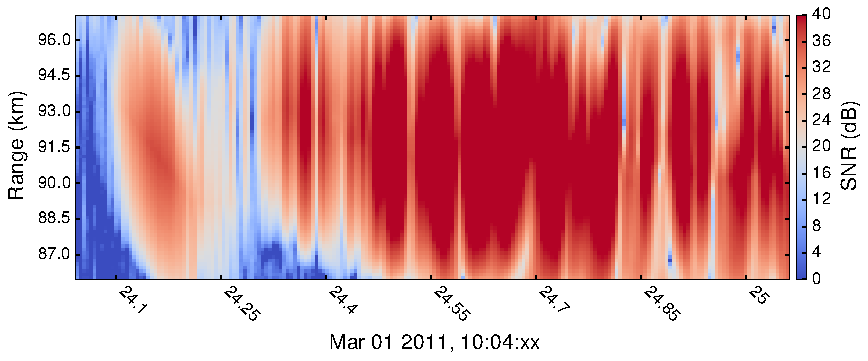
\includegraphics[trim=0px 20px 0px 3px,clip]{head_and_flare_mf_rti_2}
  \caption{Matched filter}
  \label{fig:unc_mf}
 \end{subfigure}
 
 \vspace{0.5\baselineskip}
 \begin{subfigure}{\textwidth}
  \centering
  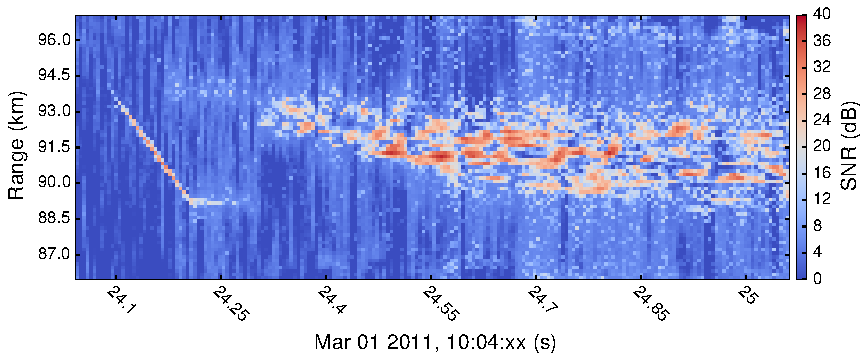
\includegraphics[trim=0px 20px 0px 3px,clip]{head_and_flare_recovered_rti_noise_2}
  \caption{Frequency-integrated waveform inversion}
  \label{fig:unc_recovered}
 \end{subfigure}
 
 \vspace{0.5\baselineskip}
 \begin{subfigure}{\textwidth}
  \centering
  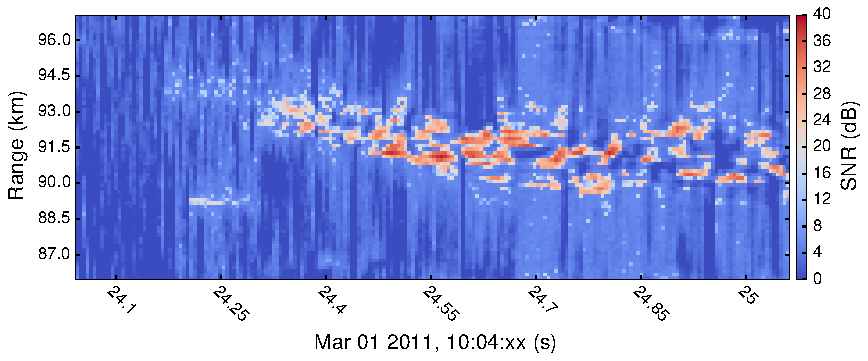
\includegraphics[trim=0px 20px 0px 3px,clip]{head_and_flare_recovered_doppler_rti_f0_p2}
  \caption{Zero-frequency slice of waveform inversion}
  \label{fig:unc_recovered_dopplerslice}
 \end{subfigure}
 \caption[Waveform inversion with the uncoded pulse]{\emph{Waveform inversion with the uncoded pulse.} Despite sidelobes that completely obscure the matched filter result, waveform inversion is successful at recovering the meteor scatter. Mismatch artifacts are also minimized in comparison to the coded pulses, producing a cleaner frequency-integrated result.}
 \label{fig:unc_comparison}
\end{figure}%
Waveform inversion successfully eliminates the sidelobes of the uncoded pulse and recovers a solution that is similar to the other waveforms. There are both negatives and positives with the uncoded pulse. On the one hand, the zero-frequency result shows that it misses some of the lower-SNR details that the other waveforms reveal in the meteor trail, and the matched filtered residual still produces prominent ghost sidelobes. On the other hand, the mismatch between the ideal waveform and its idealized model is reduced for the uncoded pulse without the complexities of coding, and the frequency-integrated result is relatively free of artifacts. It is still expected that an uncoded pulse will produce measurements that are more coherent than most codes, causing the waveform inversion to struggle in recovering denser solutions. However, the uncoded pulse has taught us that the more important consideration is waveform fidelity. Therefore, uncoded or lower-bandwidth pulses may be used if needed to ensure fidelity.

\subsection{LFM Chirp}
The LFM chirp has a very special ambiguity function; it is compact along a line in delay-frequency space, but within that line it is extremely ambiguous. As it turns out, that ambiguity is too much to overcome, and the LFM chirp is the only waveform that we tested that completely fails waveform inversion. The evidence is given in Figure \ref{fig:lfm_comparison}.
\begin{figure}[tpb]
 \vspace{-1.5\baselineskip}
 \begin{subfigure}{\textwidth}
  \centering
  \textsf{\footnotesize Mar 01 2011, 10:04:xx (s)}
  
  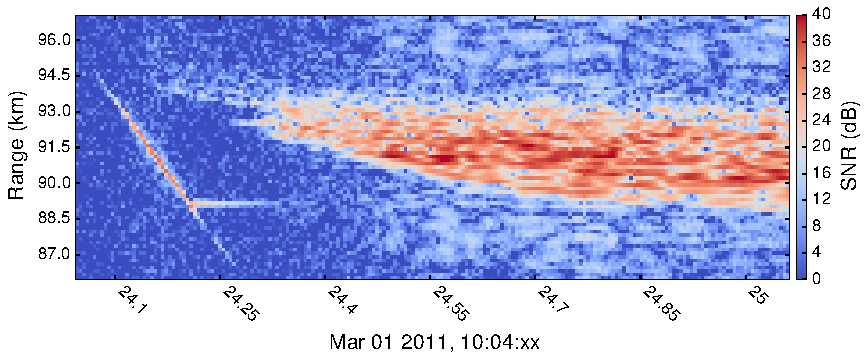
\includegraphics[trim=0px 20px 0px 3px,clip]{head_and_flare_mf_rti_3}
  \caption{Matched filter}
  \label{fig:lfm_mf}
 \end{subfigure}
 
 \vspace{0.5\baselineskip}
 \begin{subfigure}{\textwidth}
  \centering
  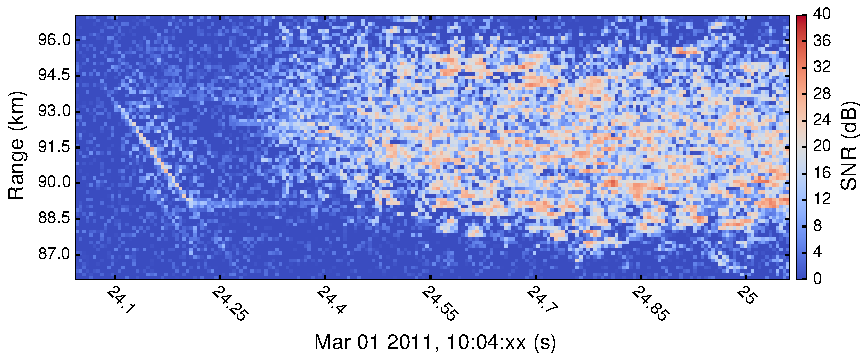
\includegraphics[trim=0px 20px 0px 3px,clip]{head_and_flare_recovered_rti_noise_3}
  \caption{Waveform inversion}
  \label{fig:lfm_recovered}
 \end{subfigure}
 \caption[Waveform inversion with the LFM chirp]{\emph{Waveform inversion with the LFM chirp.} The ridge of delay-frequency ambiguity, a defining property of the LFM chirp, makes waveform inversion impossible. The head echo gains more sidelobes but is still visible, while the trail scattering is represented by completely non-physical reflectivities.}
 \label{fig:lfm_comparison}
\end{figure}%
Without a clear delay-frequency peak produced by the matched filter bank, the sparse approximation algorithm can't pinpoint scatterers, and recovery is impossible. In the parlance of compressed sensing, the measurements are too coherent in the delay-frequency dictionary to allow for undersampling. To make matters worse, it must be noted that the radar model doesn't really accommodate the LFM chirp since it requires a discrete code with constant bauds. To perform waveform inversion (or apply digital matched filtering), the continuous frequency sweep has to be discretized. These problems should not be read as an indictment of all chirp waveforms, however. Truly discrete chirps require no special treatment, and the ridge ambiguity is only a property of the linear chirp. Judging from the ambiguity function, we expect that a quadratic or other type of chirp (e.g. an Alltop sequence) would have properties sufficient for inversion.

\subsection{Inter-waveform Comparison}
The relative performance of each of the waveforms can already be inferred by comparing the plots of each of their results, but displaying them together will make the comparison easier. We return to the second meteor example and present the waveform inversion results for the pseudorandom code, minimum sidelobe code, and uncoded pulse. These are shown in Figure \ref{fig:waveform_comparison} as frequency-integrated RTI plots and in Figure \ref{fig:waveform_comparison_doppler0} as zero-frequency slices.
\begin{figure}[tpb]
 \vspace{-1.5\baselineskip}
 \begin{subfigure}{\textwidth}
  \centering
  \textsf{\footnotesize Mar 01 2011, 10:09:xx (s)}
  
  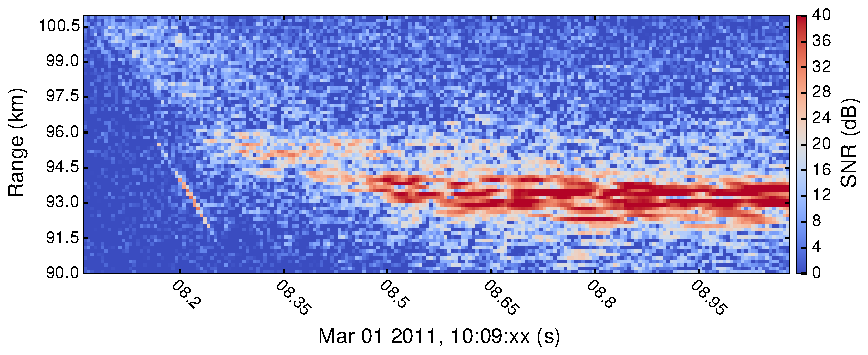
\includegraphics[trim=0px 20px 0px 3px,clip]{longtrail_recovered_rti_noise_4}
  \caption{Pseudorandom code, PSRND$_\text{51}$}
  \label{fig:longtrail_psrnd_recovered}
 \end{subfigure}
 
 \vspace{0.5\baselineskip}
 \begin{subfigure}{\textwidth}
  \centering
  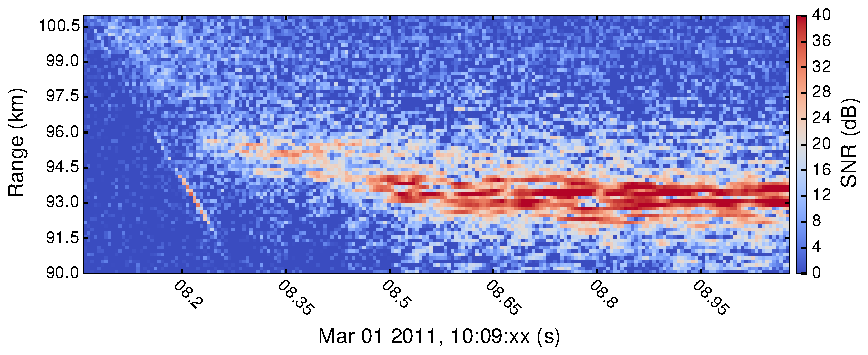
\includegraphics[trim=0px 20px 0px 3px,clip]{longtrail_recovered_rti_noise_1}
  \caption{Minimum peak sidelobe code, MSL$_\text{51}$}
  \label{fig:longtrail_msl_recovered}
 \end{subfigure}
 
 \vspace{0.5\baselineskip}
 \begin{subfigure}{\textwidth}
  \centering
  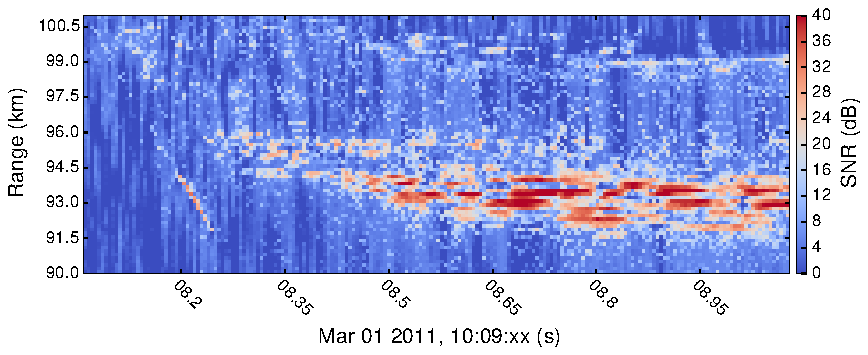
\includegraphics[trim=0px 20px 0px 3px,clip]{longtrail_recovered_rti_noise_2}
  \caption{Uncoded pulse}
  \label{fig:longtrail_unc_recovered}
 \end{subfigure}
 \caption[Frequency-integrated waveform inversions of different waveforms]{\emph{Frequency-integrated waveform inversions of different waveforms.} These images compare results for the second meteor example. They reveal that the significant signals are common to all of the waveforms, but the lower-SNR artifacts differ. This is evidence that the artifacts are related to transmitted waveform mismatch.}
 \label{fig:waveform_comparison}
\end{figure}%
\begin{figure}[tpb]
 \vspace{-1.5\baselineskip}
 \begin{subfigure}{\textwidth}
  \centering
  \textsf{\footnotesize Mar 01 2011, 10:09:xx (s)}
  
  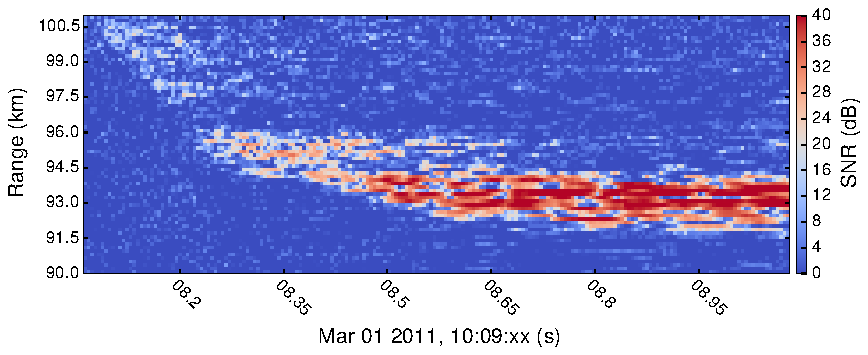
\includegraphics[trim=0px 20px 0px 3px,clip]{longtrail_recovered_doppler_rti_f0_p4}
  \caption{Pseudorandom code, PSRND$_\text{51}$}
  \label{fig:longtrail_psrnd_doppler0}
 \end{subfigure}
 
 \vspace{0.5\baselineskip}
 \begin{subfigure}{\textwidth}
  \centering
  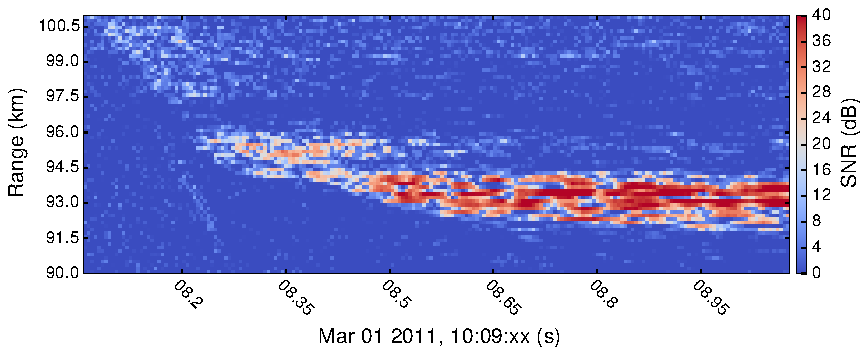
\includegraphics[trim=0px 20px 0px 3px,clip]{longtrail_recovered_doppler_rti_f0_p1}
  \caption{Minimum peak sidelobe code, MSL$_\text{51}$}
  \label{fig:longtrail_msl_doppler0}
 \end{subfigure}
 
 \vspace{0.5\baselineskip}
 \begin{subfigure}{\textwidth}
  \centering
  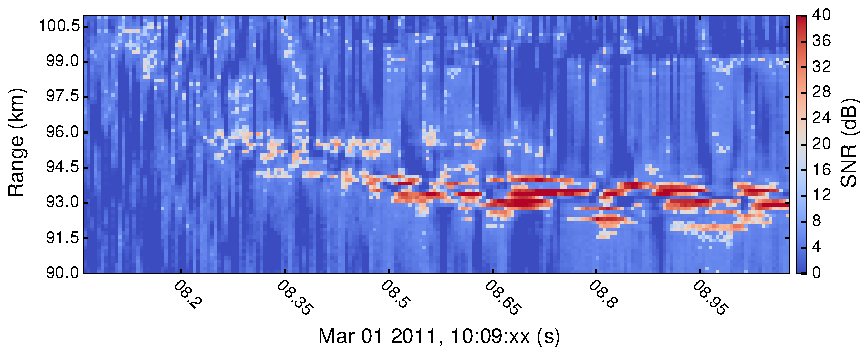
\includegraphics[trim=0px 20px 0px 3px,clip]{longtrail_recovered_doppler_rti_f0_p2}
  \caption{Uncoded pulse}
  \label{fig:longtrail_unc_doppler0}
 \end{subfigure}
 \caption[Zero-frequency waveform inversion slices of different waveforms]{\emph{Zero-frequency waveform inversion slices of different waveforms.} The coded pulses produce remarkably similar results when mismatch artifacts are not considered, while the uncoded pulse lags behind somewhat. The consistency is evidence that the results are close to the true sparse solution.}
 \label{fig:waveform_comparison_doppler0}
\end{figure}%
The comparison of these results is our basis for claiming that the artifacts present in the solution, and most noticeable in the frequency-integrated plots, are based on waveform mismatch. Each of the waveforms produces an image that agrees for the location and strength of the significant scattering. Sensitivity to low SNR scattering is more variable, but by examining the frequency slices it becomes clear which of the lower-SNR signals are true scattering and which are artifacts spread across all frequency steps. Since the form of these artifacts changes with each of the codes, they are a code-dependent property. Since the artifacts are minimized with the uncoded pulse, we conclude that they are a result of mismatch between the actual waveform and its idealized model.

The zero-frequency slices are more illuminating when it comes to revealing the recovery properties of the waveforms themselves and not that of these particular imperfect measurements. The slices clearly show that the coded pulses are strictly better than the uncoded pulse in accurately recovering the meteor trail. Significant features present in the coded pulse results are absent with the uncoded pulse, and it seems more likely that it is a failing of the latter rather than a coincidence of the former. Stripping away most of the waveform artifacts, as with these zero-frequency inversion results for the coded pulses, gives the clearest image of trail scattering that we can produce. Their degree of similarity is amazing, and it must be representative of the fact that we are getting close to the true solution.

\section{Undersampling Results}
One unexplored property of the waveform inversion method is the ability to set the model undersampling factor $R$ to a value greater than 1, which would achieve higher resolution results. The method has proven useful for sidelobe elimination, but sparsity could allow us to accomplish more by truly taking advantage of the compression aspect of compressed sensing. Theoretically, the key to recovery at increased resolution is still measurement incoherence, and the best way to likely ensure that is to increase the bandwidth of the transmitted waveform. As we have seen with the uncoded pulse, however, that is not a necessary condition for success.

\subsection{Discarding Half the Data}
In lieu of being able to validate the increased resolution with $R>1$ using the matched filter, as we have done with the previous results, we can deliberately undersample the existing data and use our full knowledge as a basis of comparison. In Figure \ref{fig:half_sampling_comparison}, we compare waveform inversion with half of the data samples (keeping every other one) to waveform inversion with the full data set.
\begin{figure}[tpb]
 \vspace{-1.5\baselineskip}
 \begin{subfigure}{\textwidth}
  \centering
  \textsf{\footnotesize Mar 01 2011, 10:04:xx (s)}
  
  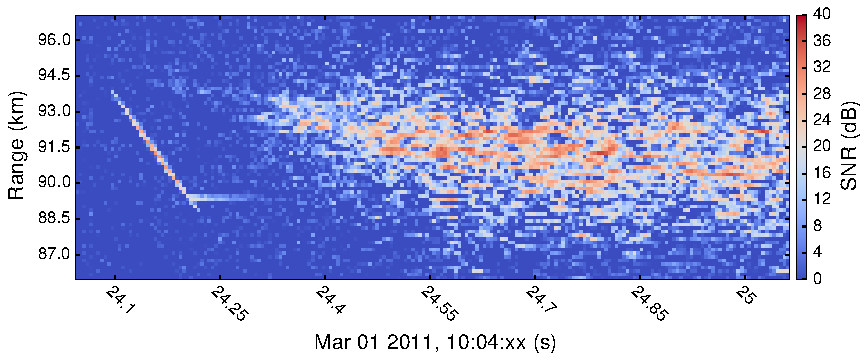
\includegraphics[trim=0px 20px 0px 3px,clip]{head_and_flare_half_recovered_rti_noise_4}
  \caption{Half the samples, frequency-integrated}
  \label{fig:half_recovered}
 \end{subfigure}
 
 \vspace{0.5\baselineskip}
 \begin{subfigure}{\textwidth}
  \centering
  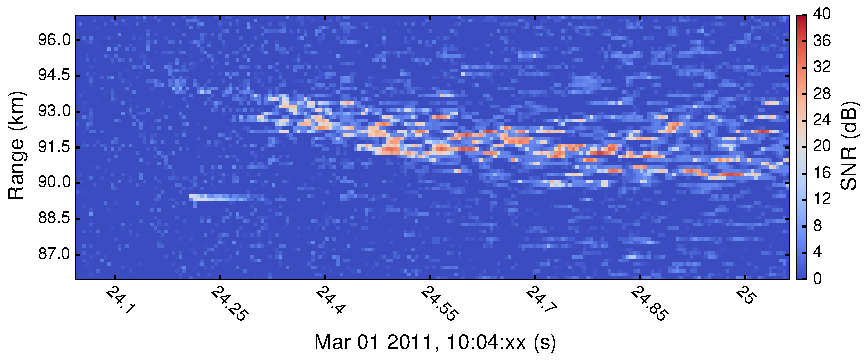
\includegraphics[trim=0px 20px 0px 3px,clip]{head_and_flare_half_recovered_doppler_rti_f0_p4}
  \caption{Half the samples, zero-frequency slice}
  \label{fig:half_recovered_doppler0}
 \end{subfigure}
 
 \vspace{0.5\baselineskip}
 \begin{subfigure}{\textwidth}
  \centering
  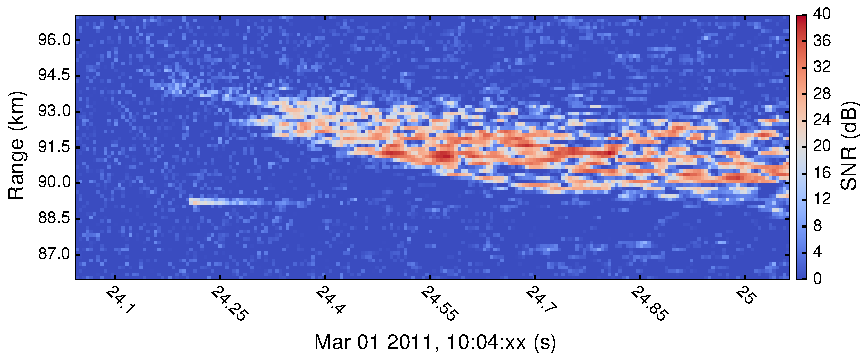
\includegraphics[trim=0px 20px 0px 3px,clip]{head_and_flare_recovered_doppler_rti_f0_p4}
  \caption{All samples, zero-frequency slice}
  \label{fig:recovered_doppler0}
 \end{subfigure}
 \caption[Waveform inversion with half the data]{\emph{Waveform inversion with half the data.} Waveform inversion was performed after discarding half of the pseudorandom pulse samples, and the results are compared to fully-sampled inversion. Head echo recovery is congruent with the previous results, but the trail is too sparse, indicating that the undersampling is too severe.}
 \label{fig:half_sampling_comparison}
\end{figure}%
Since the best waveform inversion results have been the single-frequency slices with the pseudorandom pulse, that is what we have compared between the half-sampled and fully-sampled data. Though the frequency-integrated image is rife with mismatch artifacts, overall they are not much worse than what was frequently encountered with the fully-sampled data. The zero-frequency slice tells the full story, though, and the results are mixed. With half the samples, we expect the result to have half the SNR, but much more of the signal is missing. The features with the highest SNR are still present for the most part, but the surrounding scattering with lower SNR is eliminated with half the data. However, the head echo is still recovered quite well, matching our expectations from the full data set exactly. It seems most likely that half the data is not enough to recover a signal with the number of nonzero coefficients required by the trail. Instead of the full solution, what we get is the closest sparse approximation with the maximum number of coefficients that can be recovered with the given number of measurements.

\subsection{Recovering at Double Resolution}
Even with mixed success at recovering consistent results from half-sampled data, we proceed to attempt recovery at double the resolution of the fully-sampled data. At a minimum, we hope that the head echo resolution can be increased successfully. The transmitted waveforms were sampled at their bandwidth, so doubling the model sampling rate nominally makes the waveforms ambiguous over the width of two samples. This is not necessarily an insurmountable problem, as recovery with the fully ambiguous uncoded pulse shows. A consistent theme has been that the actual waveforms don't exactly match the idealized waveforms, and in reality they do vary within the "constant" bauds of each code. To perform this double-resolution recovery, we have attempted to use the non-ideality to our advantage. Rather than doubling the length of the ideal codes by repeating each of the bauds, we simulated the effects of the transmitter's limited bandwidth by upsampling and lowpass filtering the ideal codes. The result is a double-resolution waveform that should vary in a manner similar to the actual waveform.

Figure \ref{fig:increased_resolution_comparison} shows the double-resolution recovery results for the first meteor example using the pseudorandom waveform data and the upsampled, lowpass-filtered pseudorandom code. Figure \ref{fig:longtrail_increased_resolution} shows the same for the second meteor example.
\begin{figure}[tpb]
 \vspace{-1.5\baselineskip}
 \begin{subfigure}{\textwidth}
  \centering
  \textsf{\footnotesize Mar 01 2011, 10:04:xx (s)}
  
  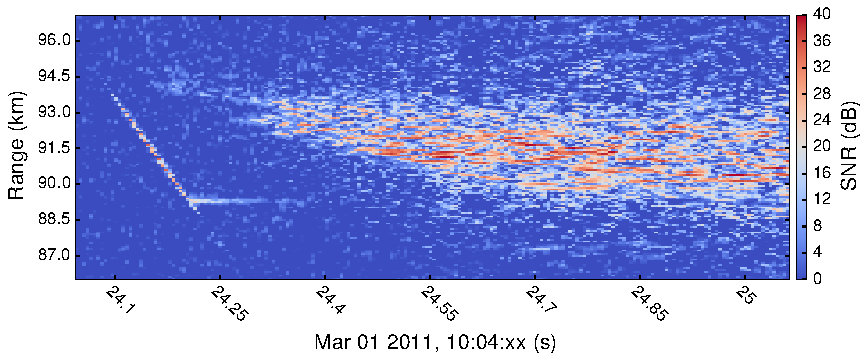
\includegraphics[trim=0px 20px 0px 3px,clip]{head_and_flare_lowpass_up_recovered_rti_noise_4}
  \caption{Double resolution, frequency-integrated}
  \label{fig:lowpass_up_recovered}
 \end{subfigure}
 
 \vspace{0.5\baselineskip}
 \begin{subfigure}{\textwidth}
  \centering
  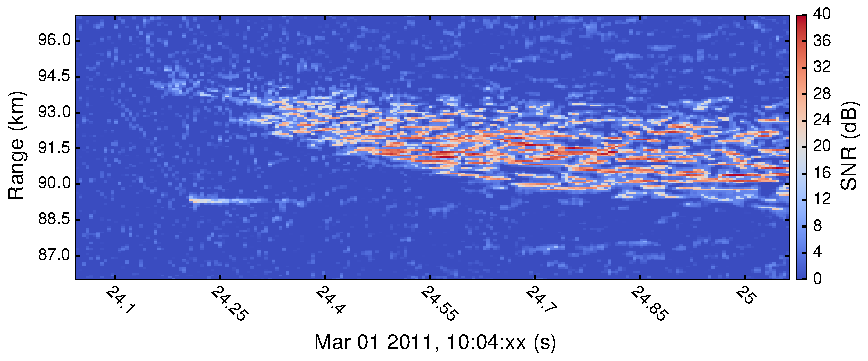
\includegraphics[trim=0px 20px 0px 3px,clip]{head_and_flare_lowpass_up_recovered_doppler_rti_f0_p4}
  \caption{Double resolution, zero-frequency slice}
  \label{fig:lowpass_up_recovered_doppler0}
 \end{subfigure}
 
 \vspace{0.5\baselineskip}
 \begin{subfigure}{\textwidth}
  \centering
  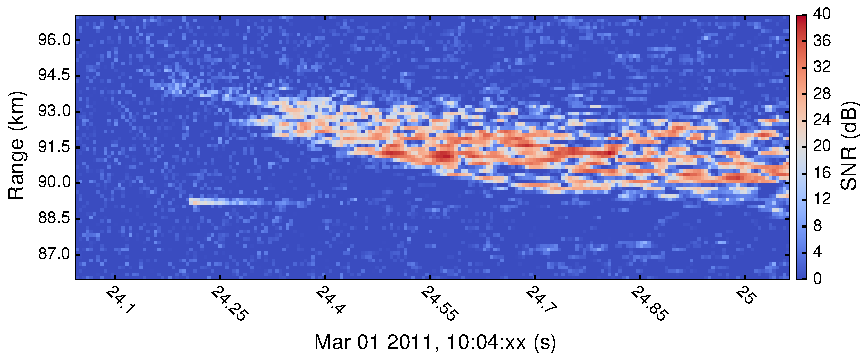
\includegraphics[trim=0px 20px 0px 3px,clip]{head_and_flare_recovered_doppler_rti_f0_p4}
  \caption{Normal resolution, zero-frequency slice}
  \label{fig:recovered_doppler0_again}
 \end{subfigure}
 \caption[Waveform inversion at double the resolution]{\emph{Waveform inversion at double the resolution.} To recover a double-resolution solution for the first meteor example, we upsampled and lowpass-filtered the pseudorandom code to simulate the effects of the actual transmitter's limited bandwidth. The results are promising, with all features represented consistently.}
 \label{fig:increased_resolution_comparison}
\end{figure}%
\begin{figure}[tpb]
 \vspace{-1.5\baselineskip}
 \begin{subfigure}{\textwidth}
  \centering
  \textsf{\footnotesize Mar 01 2011, 10:09:xx (s)}
  
  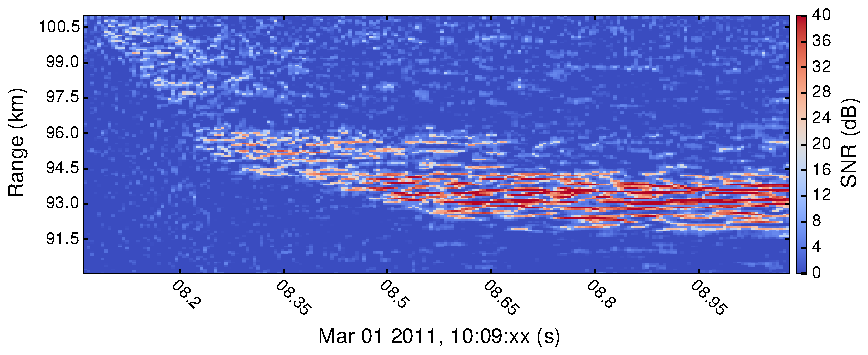
\includegraphics[trim=0px 20px 0px 3px,clip]{longtrail_lowpass_up_recovered_doppler_rti_f0_p4}
  \caption{Double resolution, frequency-integrated}
  \label{fig:psrnd_lowpass_up_doppler0}
 \end{subfigure}
 
 \vspace{0.5\baselineskip}
 \begin{subfigure}{\textwidth}
  \centering
  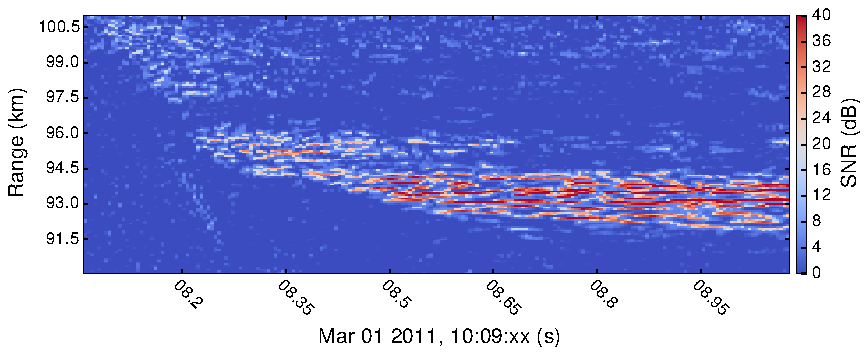
\includegraphics[trim=0px 20px 0px 3px,clip]{longtrail_lowpass_up_recovered_doppler_rti_f0_p1}
  \caption{Double resolution, zero-frequency slice}
  \label{fig:msl_lowpass_up_doppler0}
 \end{subfigure}
 
 \vspace{0.5\baselineskip}
 \begin{subfigure}{\textwidth}
  \centering
  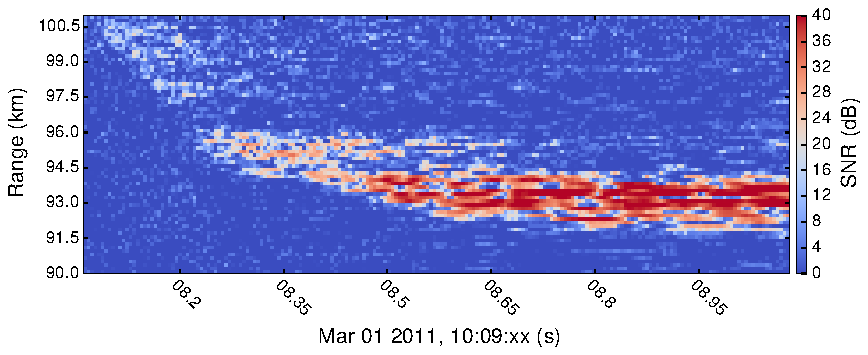
\includegraphics[trim=0px 20px 0px 3px,clip]{longtrail_recovered_doppler_rti_f0_p4}
  \caption{Normal resolution, zero-frequency slice}
  \label{fig:psrnd_doppler0}
 \end{subfigure}
 \caption[Waveform inversion at double the resolution, second example]{\emph{Waveform inversion at double the resolution, second example.} Doubling the resolution of the second meteor example also produces promising results. One can easily imagine that the normal-resolution image is a blurred version of the double-resolution image. However, it is impossible to determine whether that is truly the case.}
 \label{fig:longtrail_increased_resolution}
\end{figure}%
Whether the difference is a better relative sparsity or the fact that the lowpass-filtered code better represents the true waveform, these double resolution results \emph{look} better than the half-sampled results. In both examples, the mismatch artifacts appear to be noticeably reduced in the frequency-integrated image, and the double-resolution image has all of the same significant features as the normal-resolution image. In fact, it is easy to imagine that the original results represent a blurred version of the "true" increased-resolution results. Do the localized striations of the double-resolution trails give a better representation of the plasma and scattering physics? Without further support and given the half-sampled recovery results, it is impossible to declare victory and claim that we have successfully doubled the range resolution of our measurements. Regardless, the method looks promising and definitely merits further research.

\section{Recommendations}
\subsection{Waveform Selection}
The waveform inversion results have demonstrated the method's usefulness, eliminating sidelobes in these examples and in our additional informal testing. It works with a variety of codes, even with uncoded pulses, but the best results were achieved with the longest codes. It is impossible to replace the sensitivity provided by a long code, and with the effect of sidelobes minimized, there is no reason to not use the longest possible pulse length. The other consideration is the code itself, and on that point we have less evidence. Removing pulse length and the clearly-suboptimal uncoded and LFM chirp ambiguities from the equation, the remaining three codes seemed to find similar success. Based on our knowledge of the solution procedure as iterative matched filtering and thresholding steps, we can make the educated guess that codes with lower peak sidelobes across the entire delay-frequency space will perform better. There is obviously less work for the recovery algorithm to do when the matched filter already does a good job. Overall, the recommendation is to use long codes with minimal delay-frequency sidelobes, which are not necessarily the minimum peak range sidelobe codes.

The other waveform consideration is fidelity with the actual transmission. The most significant artifacts in the inversion result are likely an effect of mismatch between the transmitted waveform and its idealized representation in the model. The relative success of the uncoded pulse, at least with respect to artifacts, points to this conclusion. Codes should be selected knowing the bandwidth constraints and performance characteristics of the transmitter in order to ensure that the outgoing waveform is as desired. There will always be non-idealities, however, so it is recommended that one take the additional step of sampling the transmitted waveform. With transmitter samples, it is possible to use code values that most closely match the actual waveform, and thus mismatch artifacts should be minimized.

\subsection{Frequency Analysis}
Another problem we encountered is the poor frequency resolution that results from using a relatively low-frequency radar like Jicamarca. Future work could involve developing a multi-pulse inversion method, or alternatively, use a radar that operates at a higher frequency. Another possibility for increasing frequency resolution is to increase the number of frequency steps $N$ included in the radar model. Doing so can help to improve relative sparsity as discussed in Section \ref{point_target_reflectivity}, but there are limits. Larger $N$ means more unknown variables, which means proportionally longer calculations. Larger $N$ also means making the measurements more coherent in terms of the solution space, so there is a point at which increasing $N$ would result in the failure to find the true solution. For these reasons, we recommend setting $N$ as low as possible to achieve the desired frequency resolution, optimally to the minimum value of the length $L$ of the waveform code. When this is done with sufficiently long codes, the true solution is likely to still be sparse enough to permit recovery.

The ability to decompose the waveform inversion solution into different frequency slices is a real strength of the analysis method. Though a frequency-integrated plot gives a good overview of the recovered scene, the individual frequency slices can be used to identify particular targets and better-observe their details. Even when targets that scatter at different frequency shifts are present at the same ranges, waveform inversion can separate them for individual analysis. This ability is most useful for crowded radar scenes like those encountered in the equatorial ionosphere at Jicamarca. Making full use of this capability when designing waveform inversion experiments is highly recommended.

\subsection{Computation}
One final difficulty with the waveform inversion method is the time it takes to compute the recovery solution. Instead of applying the matched filter once per pulse, inversion requires, at minimum, applying it and the forward model on the order of a hundred times. Even with an efficient implementation and quick convergence, that takes a significant amount of time. Fortunately, the method as it stands now is eminently parallelizable; each pulse is processed individually, and there is no reason that they cannot be processed at the same time instead of in sequence. For larger applications, this would certainly be recommended.